
This chapter presents the validation of the platform across two test
environments: Bench and Vehicle, followed by a dedicated
verification of the mobile application and a synthesis of the overall results. 
\par For this validation, the experimental hardware utilized is the following:
\begin{itemize}
    \item uaEFI Ultra Affordable EFI\cite{rusefi_website}
    \item Raspberry Pi Zero 2W (with headers) \cite{raspizero2w}
    \item Motorola G15 \cite{motog15}
\end{itemize}

\vspace{5mm}
\begin{figure}[H]
    \centering
    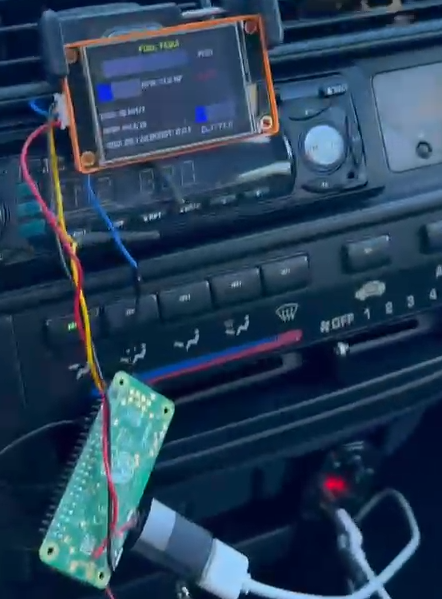
\includegraphics[width=0.35\linewidth]{imagens/hardware_photo.png}
    \caption{Hardware utilized}
    \label{fig:placeholder}
\end{figure}
\vspace{5mm}


\section{Bench Validation}

Bench validation was performed with the Raspberry Pi connected via USB serial
to a Speeduino ECU running on a static test bench, before any vehicle
integration. Each software module was verified in isolation and as part of the
integrated pipeline.
No bench validation was performed with a RusEFI ECU due to testing constraints.

The CAN acquisition pipeline was confirmed to correctly decode all signals
defined in the DBC file, including RPM, coolant temperature, MAP, TPS, AFR,
ignition advance, dwell, and battery voltage. Decoded values were cross-checked
against the reference values programmed into the ECU, with no decoding errors
observed over a 30-minute continuous run.

The \texttt{SignalCache} singleton was verified for thread-safety under
concurrent producer and consumer access. The alias synchronisation mechanism
was also validated, confirming that updates to canonical keys such as
\texttt{clt} and \texttt{advance} were correctly reflected in their aliases
\texttt{temp} and \texttt{timing}.

Database persistence was validated through a complete session lifecycle:
creation, continuous frame and signal insertion over 10 minutes, and
termination. All records were confirmed intact, and session retrieval queries
returned results in the correct order.

The BLE stack was validated using \texttt{test\_ble\_transmitter.py}, which
populated the signal cache with mock sensor data at 5~Hz and transmitted it
to the Android device. Notifications arrived at the expected 200~ms interval
with all 13 payload fields correctly received across a 20-minute streaming
session.


\section{Vehicle Validation}

Vehicle validation was performed on a road vehicle equipped with a RusEFI
ECU. The Raspberry Pi was mounted in the cabin with a CAN connection to the
ECU serial output.

Signal values from the platform were compared against TunerStudio running
simultaneously on a laptop connected to the same ECU. RPM readings matched
within $\pm$5~RPM at stable engine speeds. Coolant temperature correctly
tracked the warm-up curve from cold start to operating temperature. AFR and
EGO correction values were consistent with the closed-loop behaviour visible
in TunerStudio.

A 5-minute driving session produced approximately 5000 CAN frames stored
without write errors or data loss. Session timestamps correctly delimited the
recording window. No crashes, BLE disconnections, or process restarts were
observed throughout. CPU utilisation remained below 60\% across all concurrent
tasks.

\section{Mobile Application Verification}

The Android application was verified in three modes: mock device, bench BLE,
and vehicle BLE.

Device discovery correctly distinguished between paired-only and actively
advertising peripherals, with paired-only device cards rendered as
non-interactable. All 13 sensor fields updated correctly at 5~Hz in the live
data screen. Displayed values were validated against the bench test harness
console output and against TunerStudio during vehicle testing, with no parsing
errors or field misalignments observed.

\vspace{5mm}
\begin{figure}[H]
    \centering
    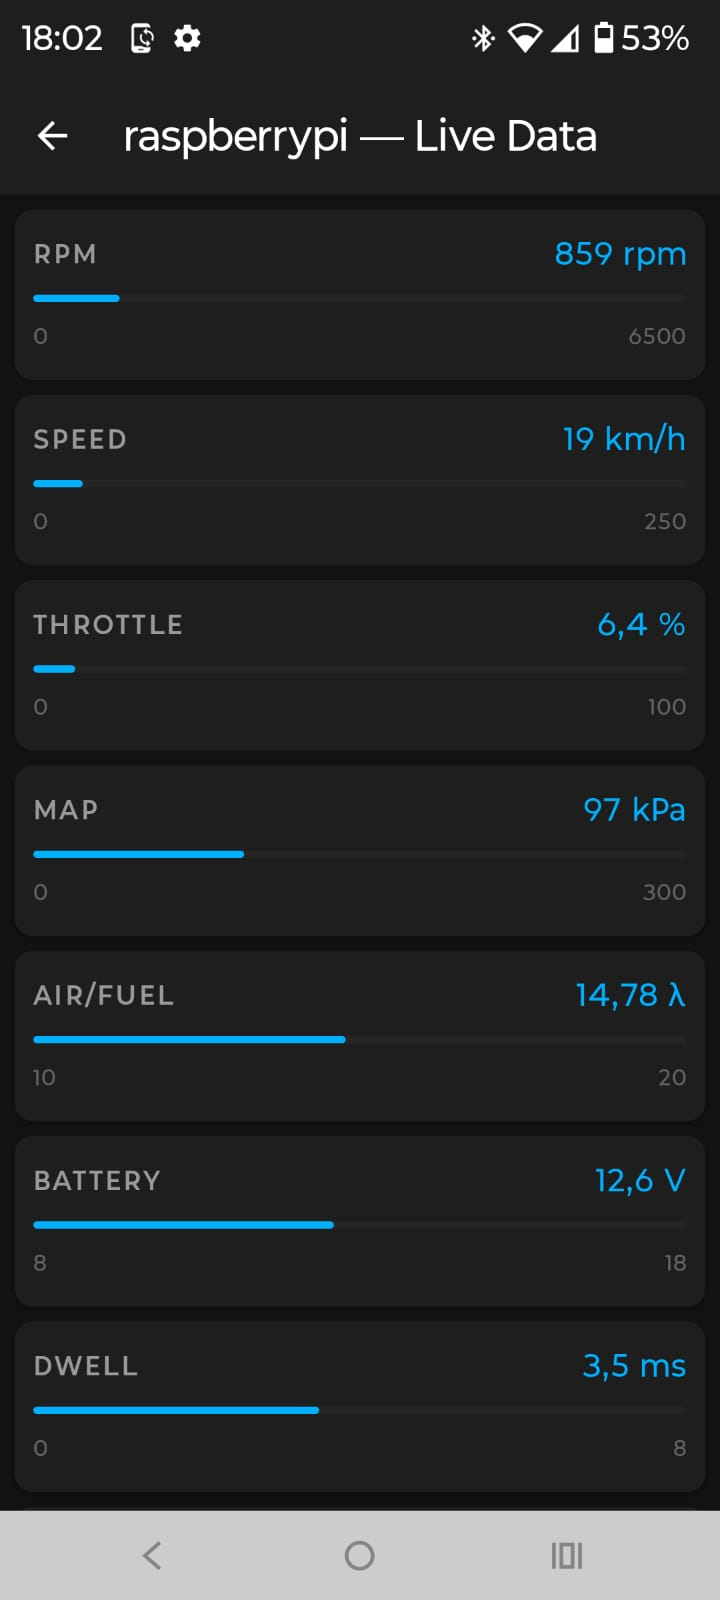
\includegraphics[width=0.35\linewidth]{imagens/mobile_test1.png}
    \caption{Live data display}
    \label{fig:placeholder}
\end{figure}
\vspace{5mm}

\clearpage
Session acquisition and start time recording were verified to be accurate,
with each driving session correctly created and timestamped upon data
collection. The session-specific statistics presented by the application were
confirmed to match the corresponding values stored in the database, indicating
that data acquisition, storage, and retrieval operated correctly throughout the
testing process.

\vspace{5mm}
\begin{figure}[H]
    \centering

    \begin{subfigure}[H]{0.35\textwidth}
        \centering
        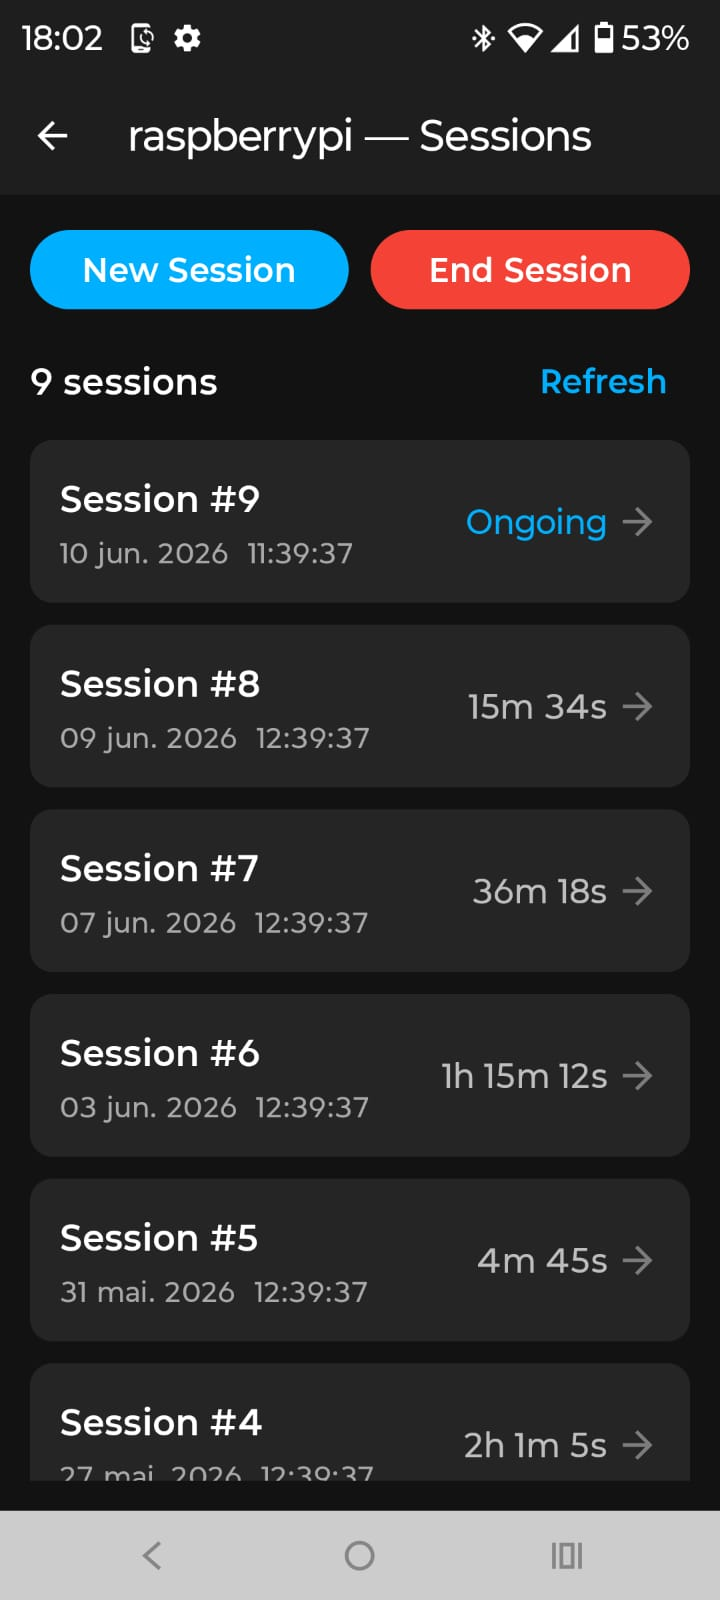
\includegraphics[width=\linewidth]{imagens/mobile_test2.png}
        \caption{Sessions display}
        \label{fig:dashboard1}
    \end{subfigure}
    \hspace{20mm}
    \begin{subfigure}[H]{0.35\textwidth}
        \centering
        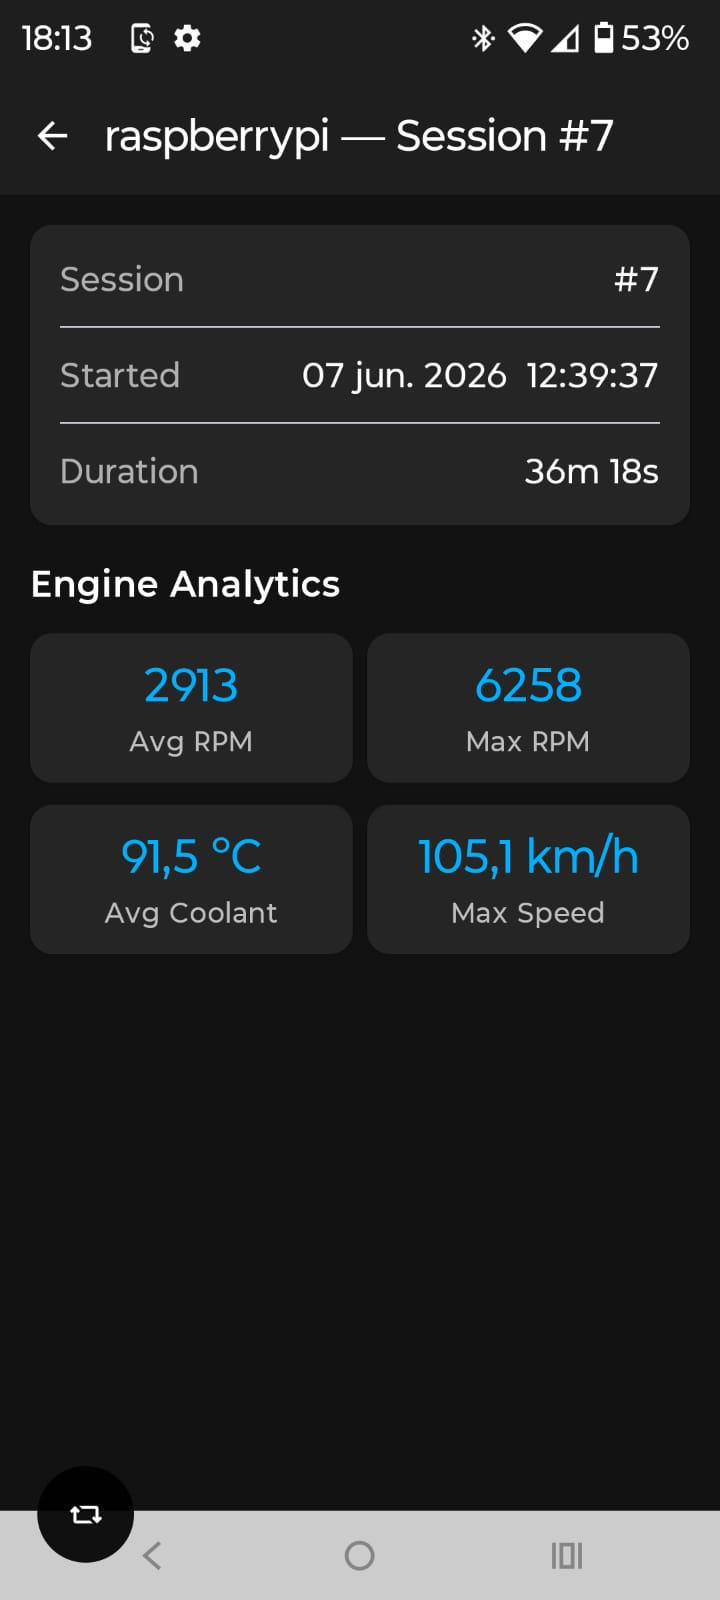
\includegraphics[width=\linewidth]{imagens/mobile_test3.png}
        \caption{Session information display}
        \label{fig:dashboard2}
    \end{subfigure}
    \caption{Session displays}
    \label{fig:dashboards}
\end{figure}
\vspace{5mm}

\clearpage

The overall statistics screen was also validated by comparing its aggregated
values with the complete set of session records stored in the database. The
application consistently displayed accurate cumulative statistics, confirming
the correctness of the aggregation logic and the integrity of the stored data.

\vspace{5mm}
\begin{figure}[H]
    \centering
    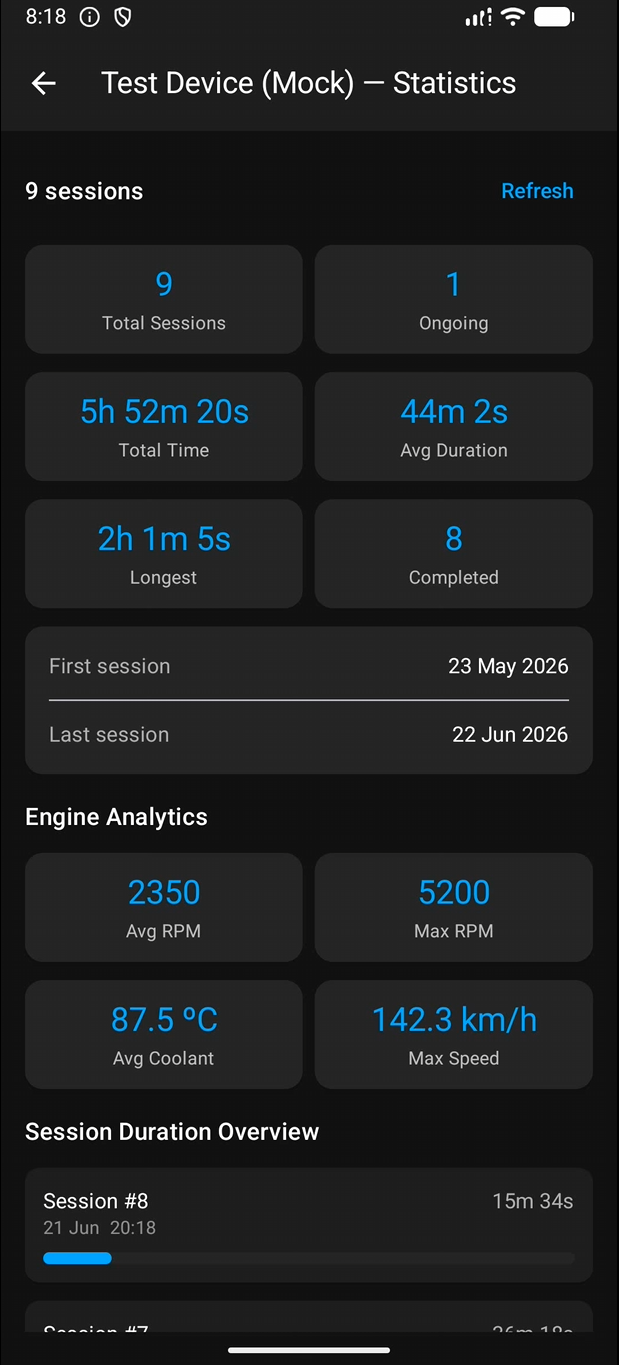
\includegraphics[width=0.35\linewidth]{imagens/mobile_test4.png}
    \caption{Overall statistics display}
    \label{fig:placeholder}
\end{figure}
\vspace{5mm}

\section{Raspberry Pi/Nextion Application verification}

The Raspberry Pi/Nextion interface was verified using both simulated and live
engine data to evaluate communication reliability, display accuracy, and user
interaction. The Nextion display was connected directly to the Raspberry Pi via
UART, while telemetry data was obtained from the shared \texttt{SignalCache}
used by the remaining platform components.

Displayed values, including RPM, coolant temperature, AFR, battery voltage,
manifold pressure, ignition timing, and throttle position, were compared
against the simulated data send or information seen on TunerStudio. All monitored 
signals were updated correctly with no observable inconsistencies between the 
displayed and transmitted data.

Screen navigation and touch interactions were validated across all available
pages. User inputs were correctly interpreted by the Raspberry Pi application,
and page transitions occurred without delays or communication errors. Extended
runtime testing was performed over a continuous 30-minute session, during which
no freezes, application crashes, or UART communication failures were observed.

The refresh rate was sufficient to provide smooth real-time feedback while
maintaining relatively low CPU utilisation on the Raspberry Pi. Throughout vehicle
operation, sensor values remained responsive to engine speed and load changes,
confirming the suitability of the interface for real-time driver monitoring.

Overall, the Raspberry Pi/Nextion subsystem operated reliably and provided an
accurate representation of the acquired ECU data, validating its integration
within the proposed platform.

\section{Results Summary}

Validation confirmed that the platform meets its primary objectives. 
CAN acquisition and DBC-based decoding operated correctly under real 
engine conditions. Continuous datalogging handled
high-frequency writes without data loss. BLE transmission reliably delivered
a 13-signal payload at 5~Hz, and the mobile application correctly displayed
all fields.

The main limitation identified is the absence of automatic BLE reconnection
logic on both the controller and the Android client, currently requiring
manual intervention after an unexpected disconnection. This is the primary
target for improvement in future iterations of the platform.


